\documentclass[a4paper,12pt]{article}
\usepackage{amsmath}
\usepackage{graphicx}
\usepackage{float}
\usepackage[a4paper, top=0.5in, bottom=0.5in, left=1in, right=1in]{geometry}
\usepackage{xcolor}
\usepackage{colortbl}
\usepackage{titlesec}
\usepackage{fontspec}
\usepackage{tikz}
\usepackage{lipsum} % For dummy text, remove this for your actual report
\usepackage{listings}
\lstset{
    language=Python,        % Specify the language
    basicstyle=\ttfamily,   % Basic font style
    keywordstyle=\color{blue}\bfseries, % Keywords style
    commentstyle=\color{green},         % Comments style
    stringstyle=\color{red},            % Strings style
    numbers=left,                      % Add line numbers
    numberstyle=\tiny,                 % Line number style
    stepnumber=1,                      % Step between line numbers
    frame=single,                      % Add a frame around the code
    breaklines=true                    % Allow breaking long lines
}
% Define colors
\definecolor{myblue}{rgb}{0.1, 0.2, 0.7}
\definecolor{mygreen}{rgb}{0.1, 0.6, 0.1}
\definecolor{myred}{rgb}{0.7, 0.2, 0.2}
\definecolor{lightblue}{rgb}{0.8, 0.9, 1}
\definecolor{mygold}{rgb}{0.8, 0.6, 0.1}
\definecolor{mygray}{rgb}{0.9, 0.9, 0.9}

% Customize title formatting
\titleformat{\title}[block]
  {\normalfont\Huge\bfseries\color{myblue}}{}{0em}{}

\titleformat{\author}[block]
  {\normalfont\LARGE\itshape\color{mygreen}}{}{0em}{}

% Custom header line
\newcommand{\myheader}{
    \noindent\rule{\textwidth}{1pt}\\[0.4cm]
}

% Title page design
\begin{document}

% Title Page
\begin{titlepage}
    \centering
    
    
    \vspace*{2cm}
    
    % Title
    {\Huge \bfseries \textcolor{myblue}{Lab Report: Oscilloscope and Function Generator}}\\[0.5cm]
    {\LARGE \textit{\textcolor{myred}{Including Lissajous Figures}}}\\[1.5cm]
    
    % Author names
    \noindent
    \textbf{\Huge Krishna Patil-EE24BTECH11036}\\[0.3cm]
    \textbf{\Huge Deepak Ahirwar-EE24BTECH11014}\\[1.5cm]
    
    % Institution name
    {\LARGE \textit{Electrical Department, IIT-Hyderabad}}\\[2cm]
    
    \vfill
    
    % Date
    {\LARGE \today}
    
    % Footer - with gradient line and custom footer text
    \vfill
    \myheader
    \centering
    \textcolor{mygold}{\Large \textit{Experiment conducted as part of EE Laboratory Coursework.}}

    
\end{titlepage}

% Content starts on next page
\newpage

\section*{\color{myblue}Objective}
\begin{enumerate}
    \item To understand the working principles of an oscilloscope and function generator.
    \item To study and observe Lissajous figures on a Cathode Ray Oscilloscope (CRO).
    \item To justify the observed Lissajous patterns with theoretical principles.
    \item To demonstrate how to capture a one-time event on a CRO.
\end{enumerate}

\section*{\color{myblue}Apparatus Required}
\begin{itemize}
    \item Cathode Ray Oscilloscope (CRO)
    \item Function Generator
    \item Connecting wires
    \item Patch cords and probes
\end{itemize}

\section*{\color{myblue}Theory}

\subsection*{\color{mygreen}Oscilloscope}
An oscilloscope is an electronic test instrument used to display and analyze the waveform of electronic signals. It allows visualization of:
\begin{itemize}
    \item Voltage versus time (in the Time Domain mode)
    \item Voltage versus another voltage (in X-Y mode, useful for Lissajous figures)
\end{itemize}

\subsection*{\color{mygreen}Function Generator}
A function generator produces electrical waveforms, such as sine, square, and triangular waves, over a wide range of frequencies.

\subsection*{\color{mygreen}Lissajous Figures}
Lissajous figures are graphical representations of parametric equations:
\[
x = A \sin(\omega_x t + \phi_x), \quad y = B \sin(\omega_y t + \phi_y)
\]
\begin{itemize}
    \item $A$ and $B$: Amplitudes of the signals
    \item $\omega_x$ and $\omega_y$: Angular frequencies
    \item $\phi_x$ and $\phi_y$: Phase angles
\end{itemize}

When these signals are fed into the X and Y inputs of a CRO in X-Y mode, the resulting patterns are Lissajous figures. The shape depends on:
\begin{enumerate}
    \item The frequency ratio $\left(\frac{\omega_x}{\omega_y}\right)$.
    \item The phase difference $\Delta\phi = \phi_x - \phi_y$.
\end{enumerate}

\subsection*{\color{mygreen}Frequency Ratio ($f_x : f_y$)}
\begin{itemize}
    \item $f_x : f_y = 1:1$: Circular or elliptical figures.
    \item $f_x : f_y = 1:2$: Two loops in the vertical direction.
    \item $f_x : f_y = 2:1$: Two loops in the horizontal direction.
    \item $f_x : f_y = m:n$: Complex figures with $m$ vertical and $n$ horizontal intersections.
\end{itemize}

\subsection*{\color{mygreen}Phase Difference ($\Delta\phi$)}
\begin{itemize}
    \item $0^\circ$: Line at $45^\circ$.
    \item $90^\circ$: Circle (if amplitudes are equal).
    \item $180^\circ$: Line at $135^\circ$.
\end{itemize}

\section*{\color{myblue}Procedure}

\subsection*{\color{myred}Setup}
\begin{enumerate}
    \item Connect the output terminals of the function generator to the CRO.
    \item Configure the CRO:
    \begin{itemize}
        \item Select the X-Y mode for Lissajous figures.
        \item Adjust the intensity, focus, and time/div knobs for clear visibility.
    \end{itemize}
    \item Use the function generator to provide two sinusoidal signals of adjustable frequency and phase.
\end{enumerate}

\subsection*{\color{myred}Observing Lissajous Figures}
\begin{enumerate}
    \item Set the horizontal (X-axis) frequency to $f_x$ and the vertical (Y-axis) frequency to $f_y$.
    \item Observe and sketch Lissajous patterns for different ratios ($1:1$, $1:2$, $2:1$, $m:n$).
    \item Fix $f_x = f_y$ and gradually change the phase difference ($0^\circ$, $90^\circ$, $180^\circ$). Note how the shape evolves.
\end{enumerate}

\section*{\color{myblue}Observations}

\begin{table}[H]
\centering
\arrayrulecolor{mygreen}\arrayrulewidth=1pt
\begin{tabular}{|c|c|c|c|}
\hline
\rowcolor{mygray} \textbf{$f_x : f_y$} & \textbf{$\Delta\phi$} & \textbf{Observed Pattern} & \textbf{Justification} \\\hline 
1:1 & $0^\circ$ & Line at $45^\circ$ & Equal frequencies, no phase lag. \\\hline
1:1 & $90^\circ$ & Circle & Orthogonal signals with equal amplitude. \\\hline
1:2 & $0^\circ$ & Two vertical loops & Double frequency on Y-axis. \\\hline
2:1 & $0^\circ$ & Two horizontal loops & Double frequency on X-axis. \\\hline
9:7 & $0^\circ$ & Complex figure & nine vertical and seven horizontal intersections. \\\hline
9:7 & $30^\circ$ & Complex figure & nine vertical and seven horizontal intersections. \\\hline
\end{tabular}
\caption{\color{myblue}Observation Table for Lissajous Figures}
\end{table}

\section*{\color{myblue}Lissajous Figures}
\begin{figure}[H]
    \centering
    \begin{subfigure}{\textwidth}
        \centering
        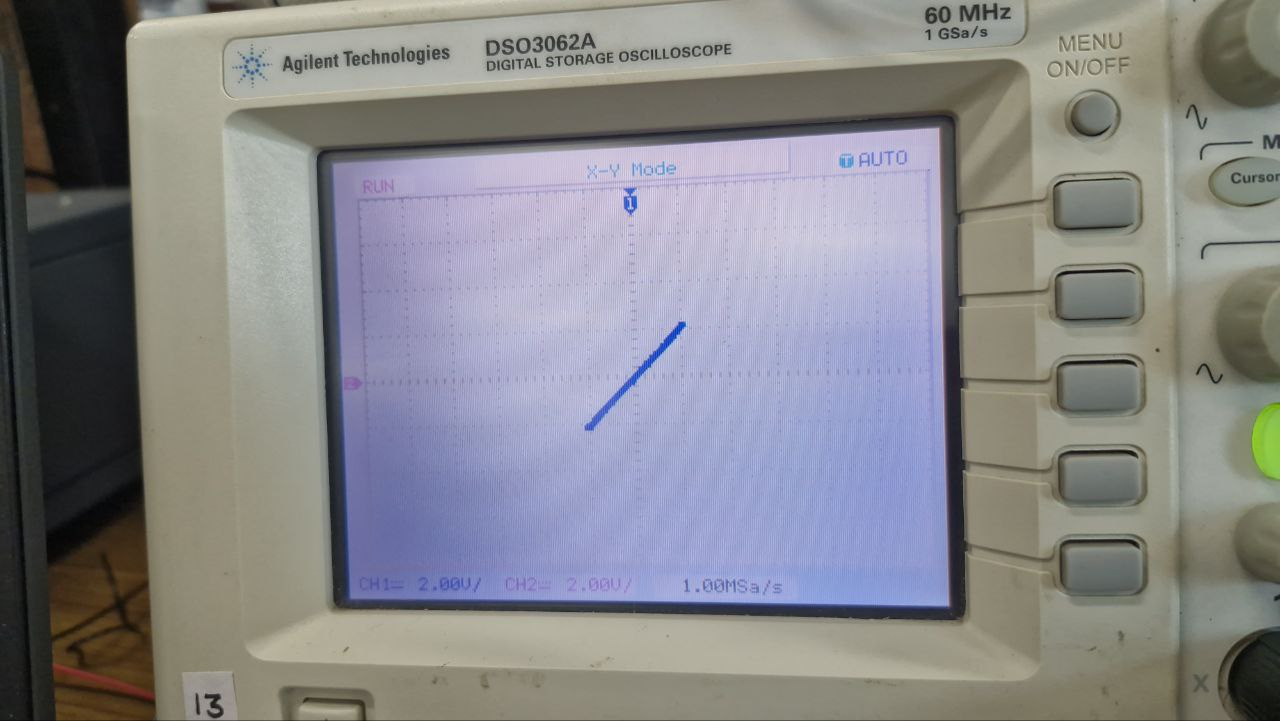
\includegraphics[height=5cm]{figures/1/plot.jpg}
    \end{subfigure}%
    \begin{subfigure}{\textwidth}
        \centering
        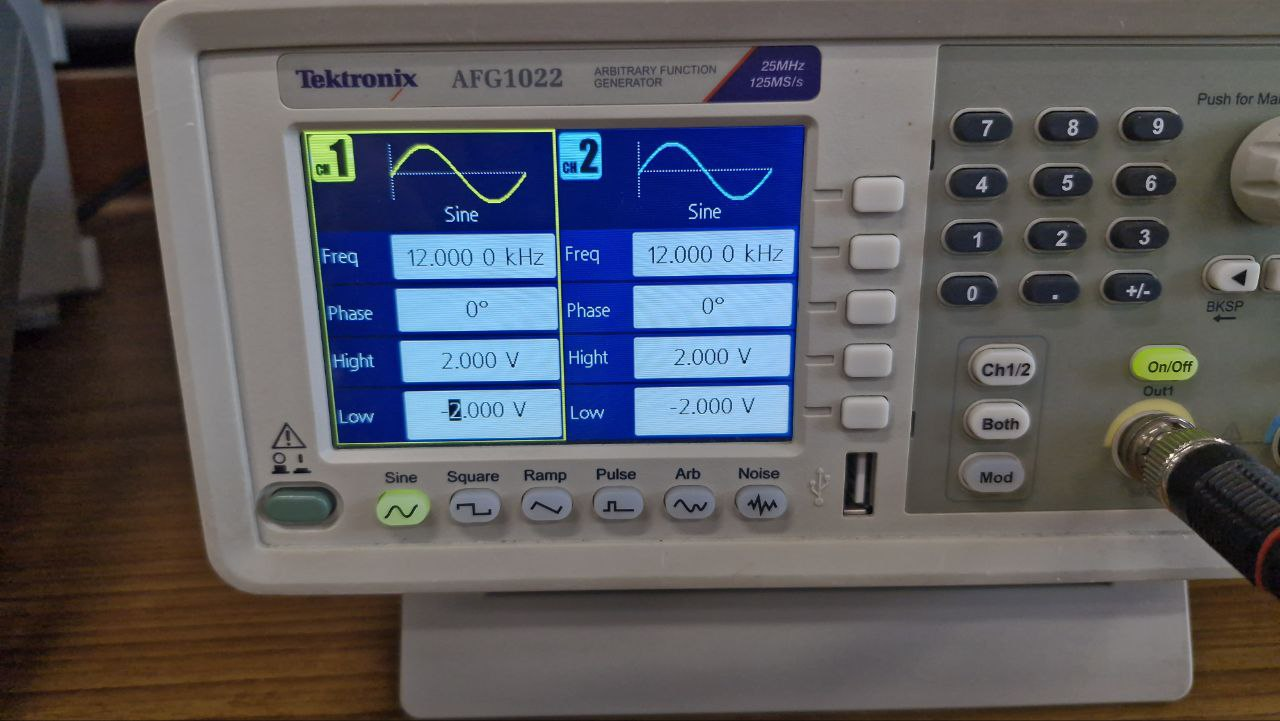
\includegraphics[height=5cm]{figures/1/para.jpg}
    \end{subfigure}
    \begin{subfigure}{\textwidth}
        \centering
        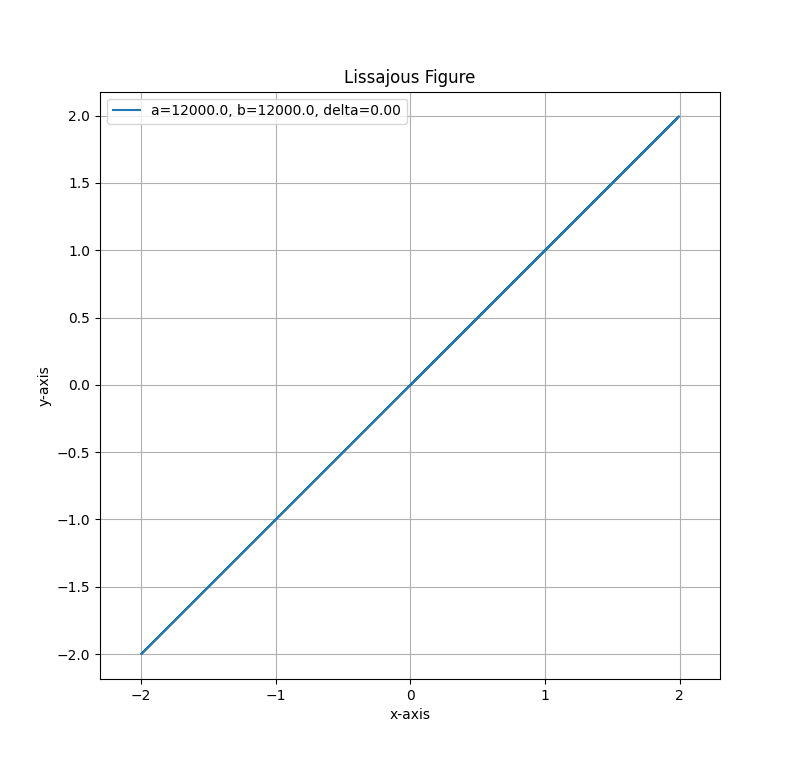
\includegraphics[height=5cm]{figures/1/Figure_1.png}
    \end{subfigure}%
\end{figure}
\begin{figure}[H]
    \centering
    \begin{subfigure}{\textwidth}
        \centering
        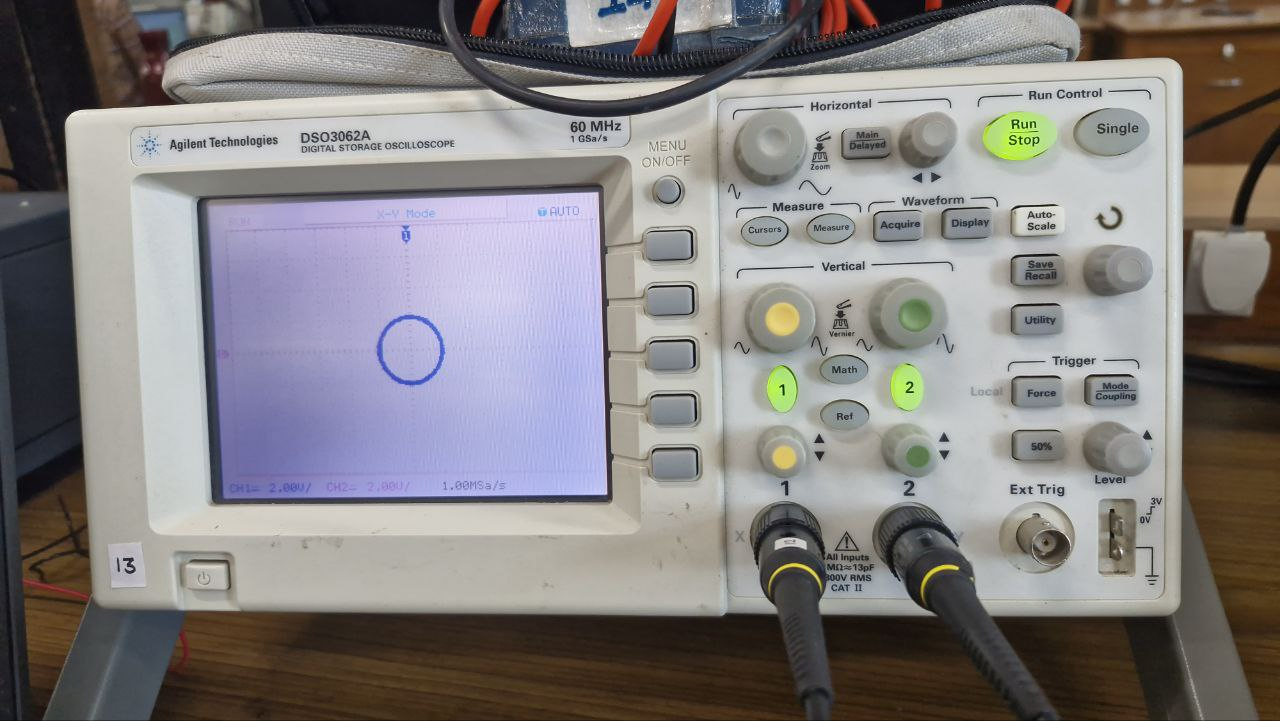
\includegraphics[height=5cm]{figures/2/plot.jpg}
    \end{subfigure}%
    \begin{subfigure}{\textwidth}
        \centering
        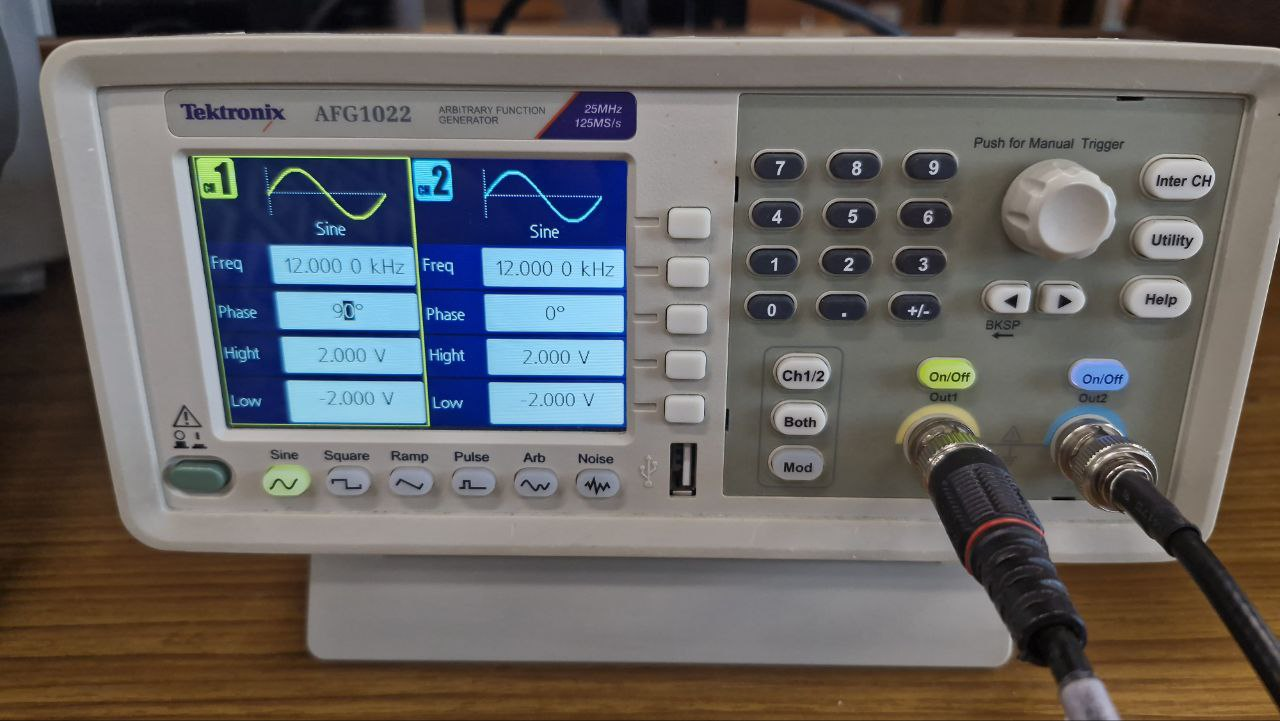
\includegraphics[height=5cm]{figures/2/para.jpg}
    \end{subfigure}
    \begin{subfigure}{\textwidth}
        \centering
        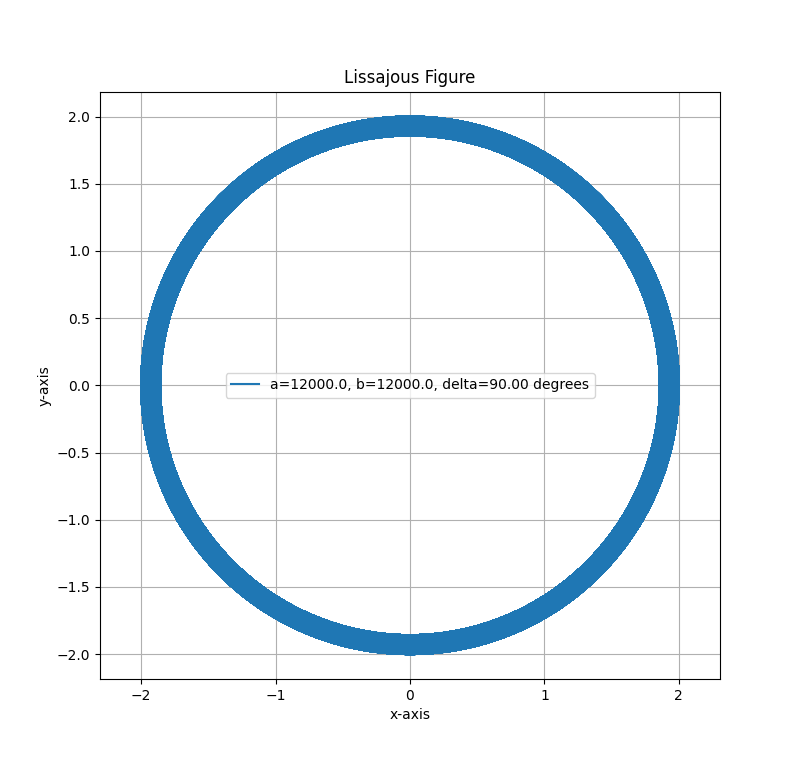
\includegraphics[height=5cm]{figures/2/Figure_2.png}
    \end{subfigure}%
\end{figure}
\begin{figure}[H]
    \centering
    \begin{subfigure}{\textwidth}
        \centering
        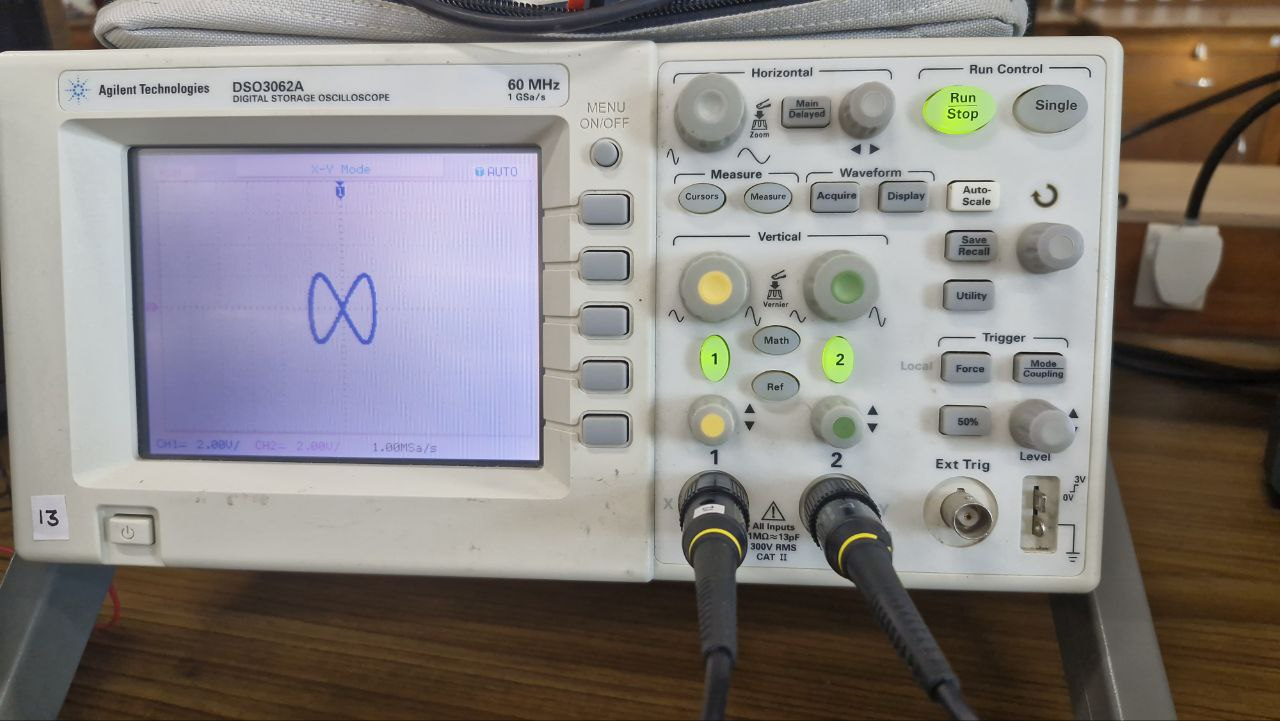
\includegraphics[height=5cm]{figures/3/plot.jpg}
    \end{subfigure}%
    \begin{subfigure}{\textwidth}
        \centering
        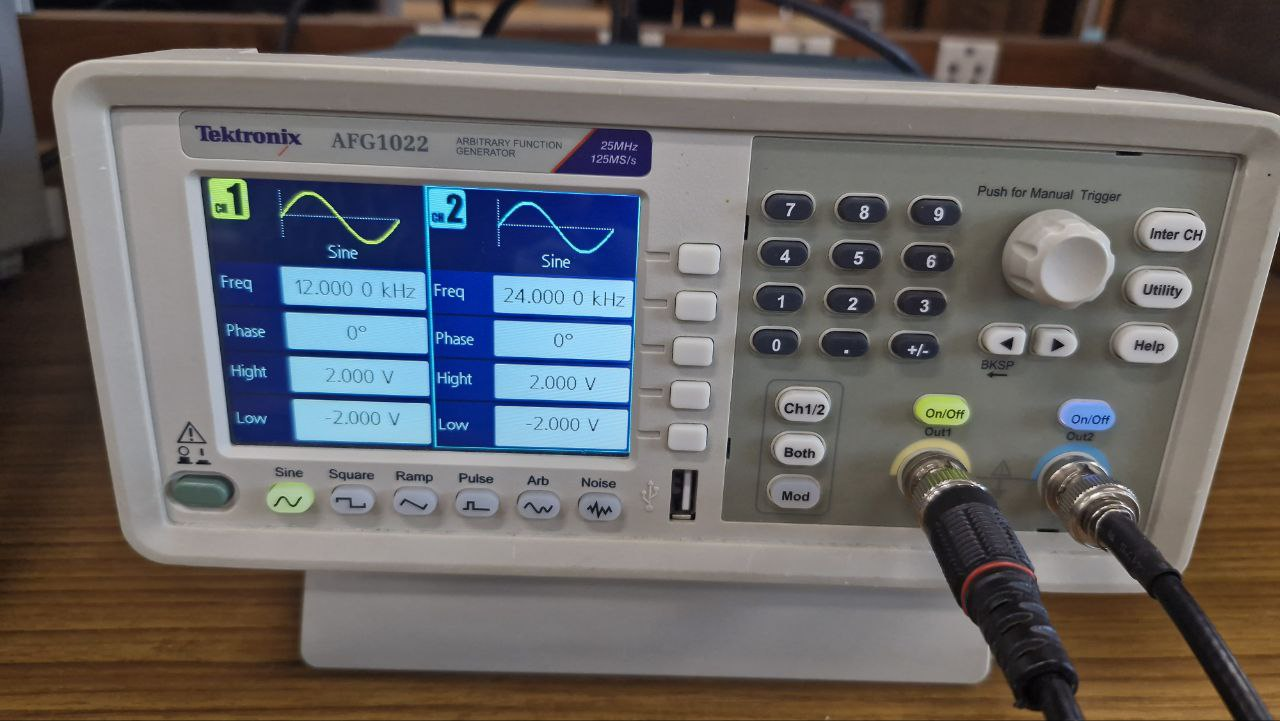
\includegraphics[height=5cm]{figures/3/para.jpg}
    \end{subfigure}
    \begin{subfigure}{\textwidth}
        \centering
        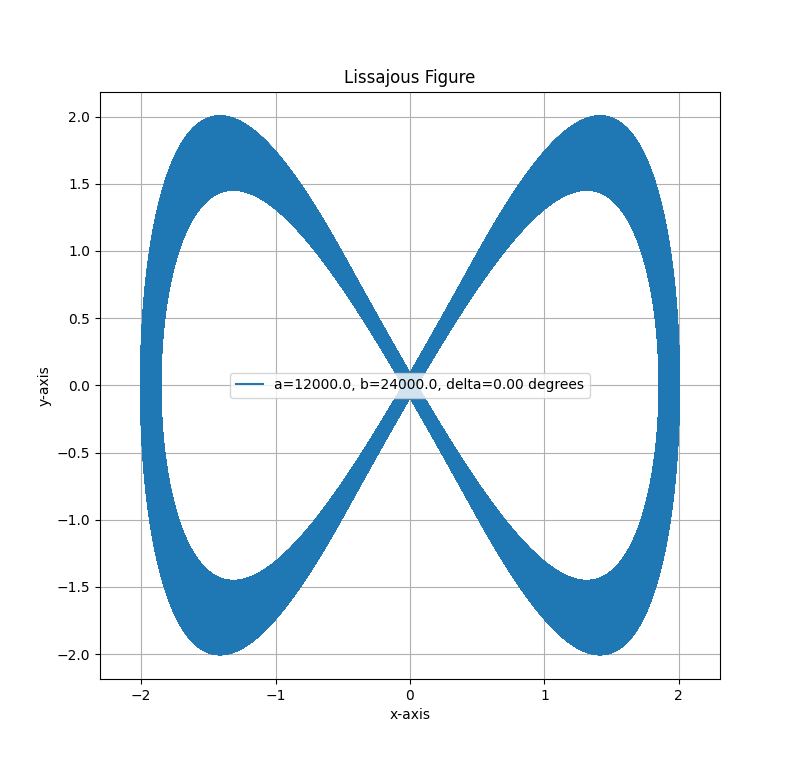
\includegraphics[height=5cm]{figures/3/Figure_3.png}
    \end{subfigure}%
\end{figure}
\begin{figure}[H]
    \centering
    \begin{subfigure}{\textwidth}
        \centering
        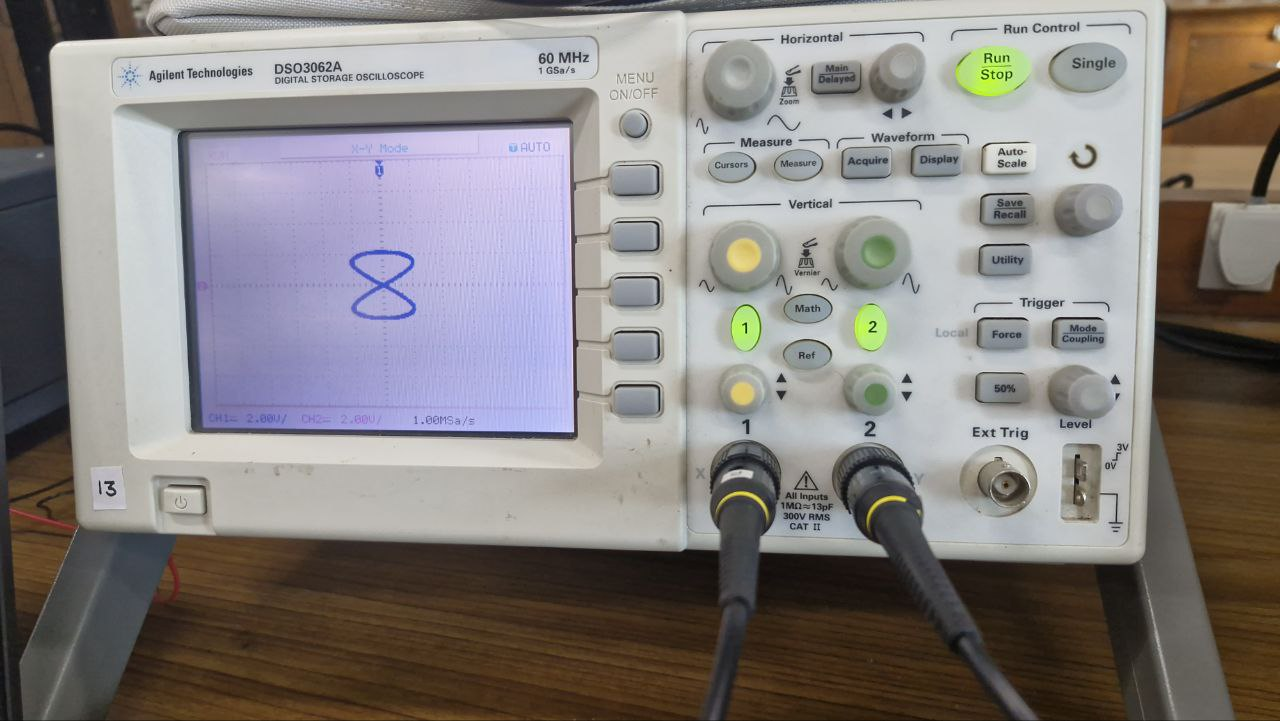
\includegraphics[height=5cm]{figures/4/plot.jpg}
    \end{subfigure}%
    \begin{subfigure}{\textwidth}
        \centering
        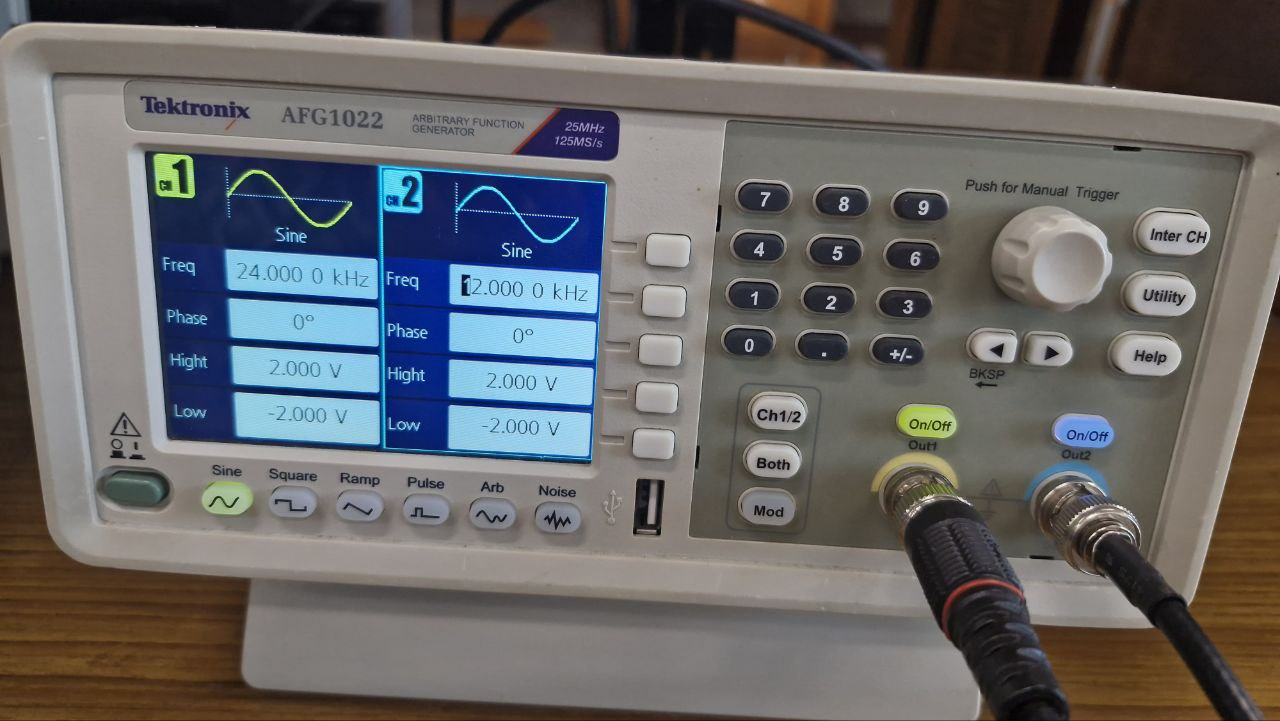
\includegraphics[height=5cm]{figures/4/para.jpg}
    \end{subfigure}
    \begin{subfigure}{\textwidth}
        \centering
        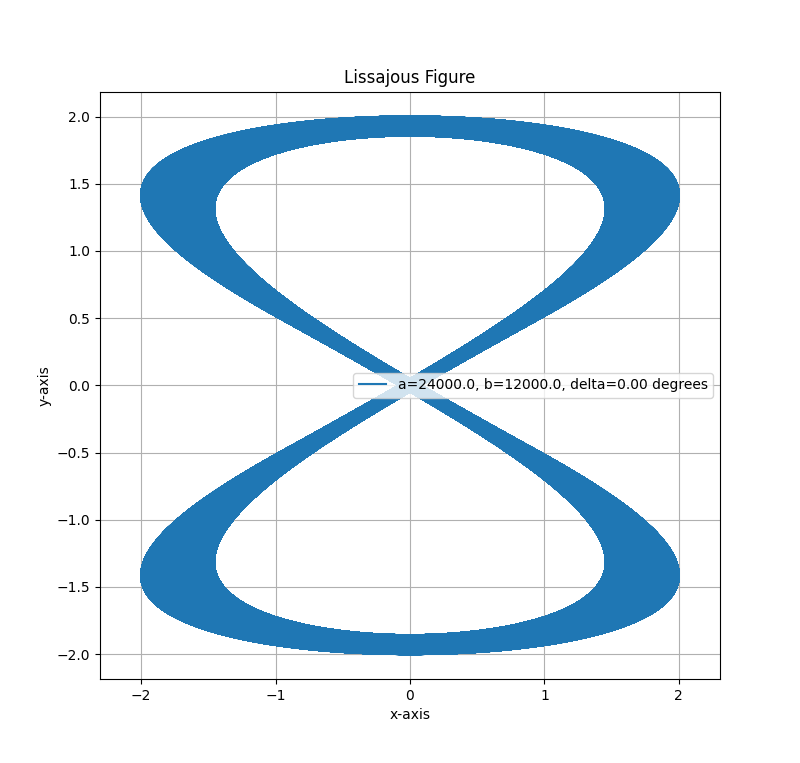
\includegraphics[height=5cm]{figures/4/Figure_4.png}
    \end{subfigure}%
\end{figure}
\begin{figure}[H]
    \centering
    \begin{subfigure}{\textwidth}
        \centering
        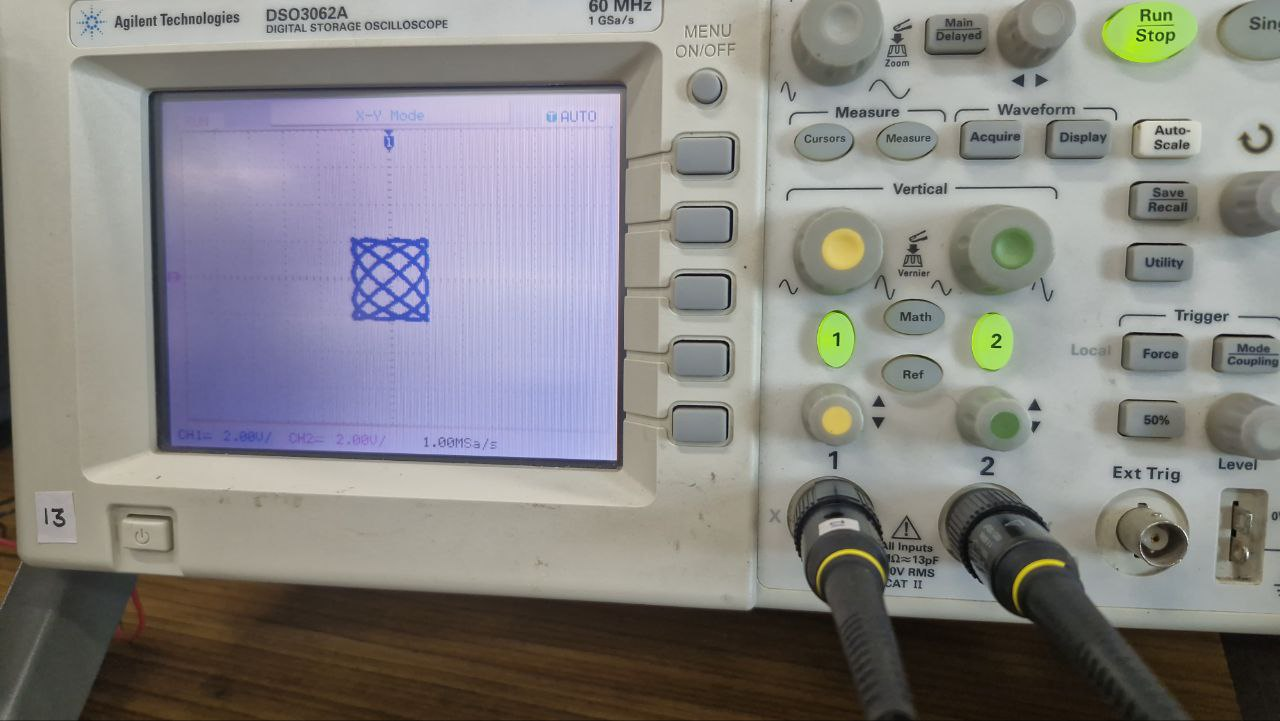
\includegraphics[height=5cm]{figures/5/plot.jpg}
    \end{subfigure}%
    \begin{subfigure}{\textwidth}
        \centering
        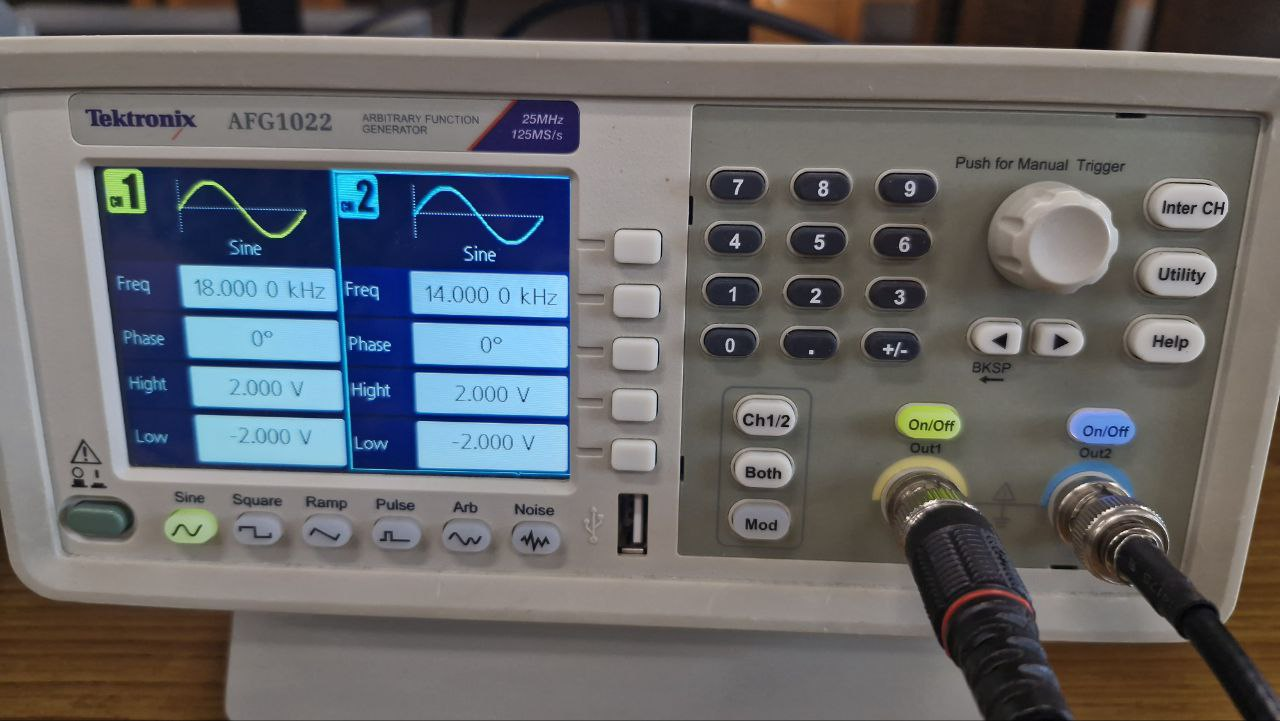
\includegraphics[height=5cm]{figures/5/para.jpg}
    \end{subfigure}
    \begin{subfigure}{\textwidth}
        \centering
        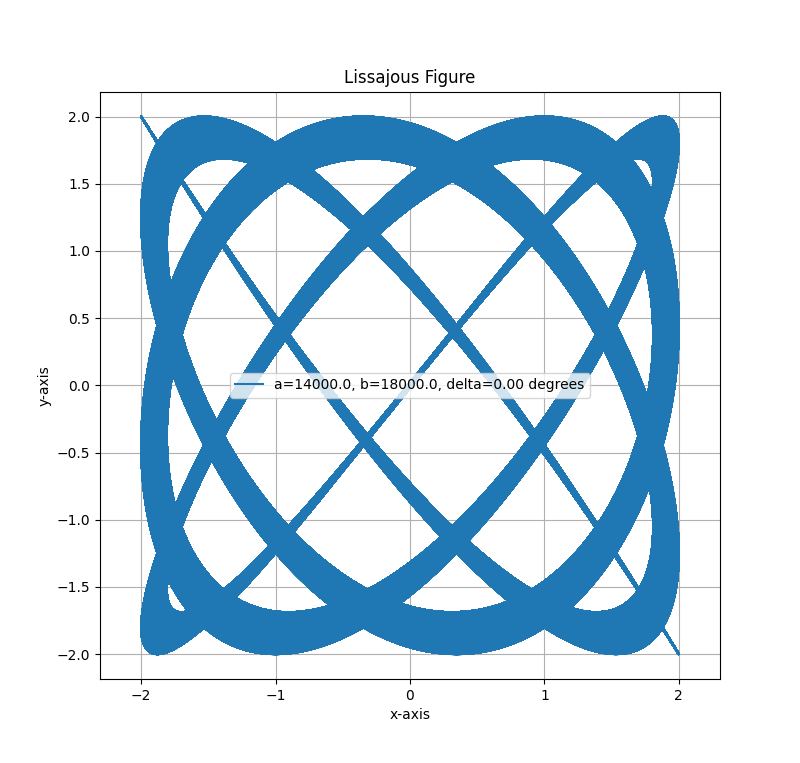
\includegraphics[height=5cm]{figures/5/Figure_5.png}
    \end{subfigure}%
\end{figure}
\begin{figure}[H]

    \centering
    \begin{subfigure}{\textwidth}
        \centering
        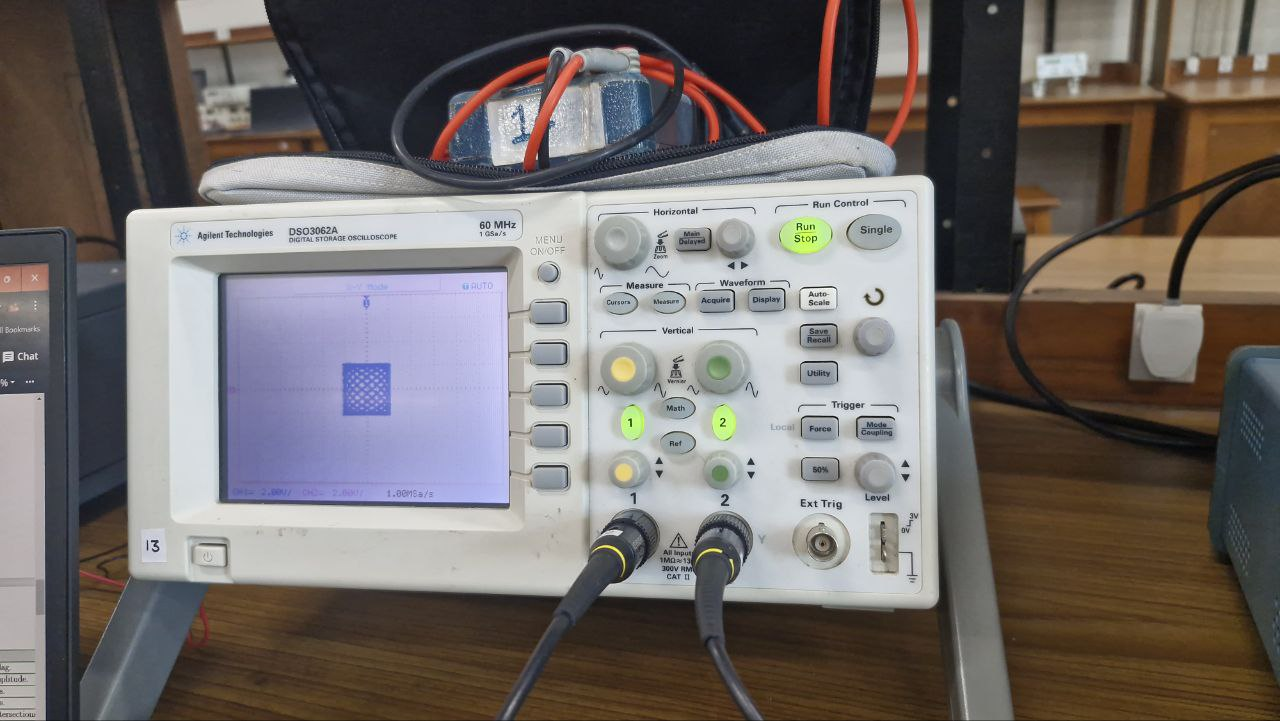
\includegraphics[height=5cm]{figures/6/plot.jpg}
    \end{subfigure}%
    \begin{subfigure}{\textwidth}
        \centering
        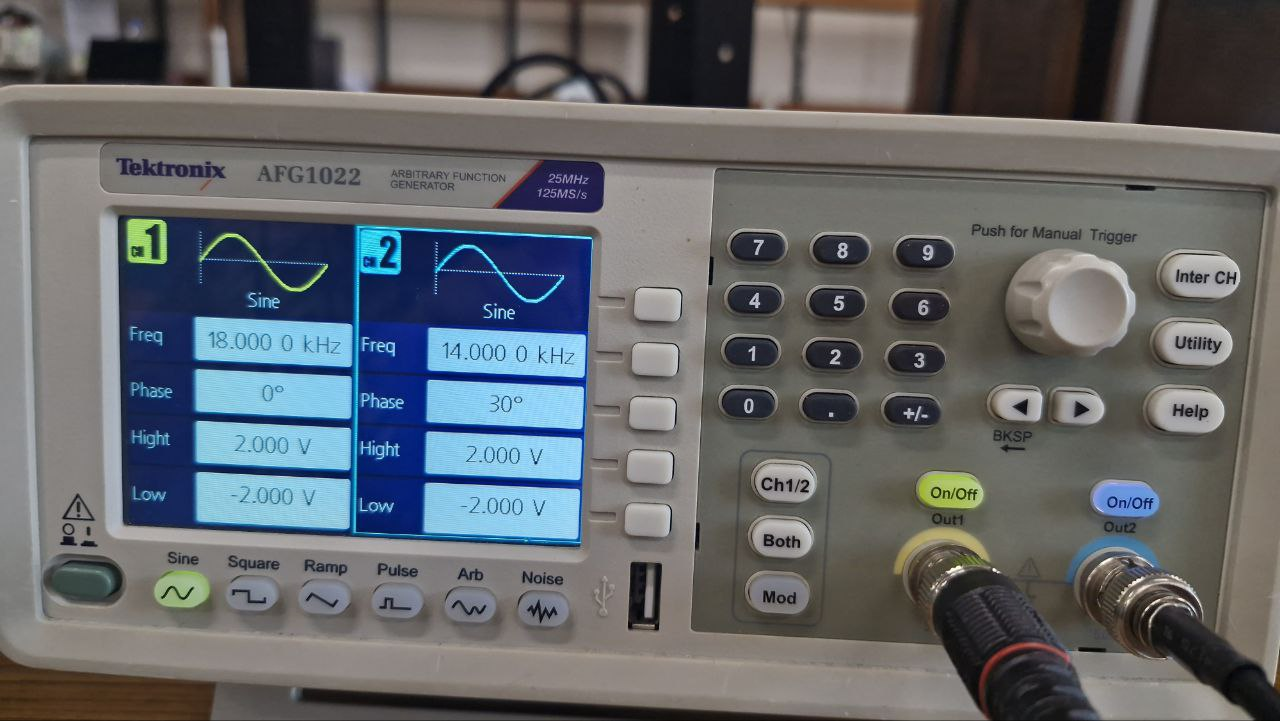
\includegraphics[height=5cm]{figures/6/para.jpg}
    \end{subfigure}
    \begin{subfigure}{\textwidth}
        \centering
        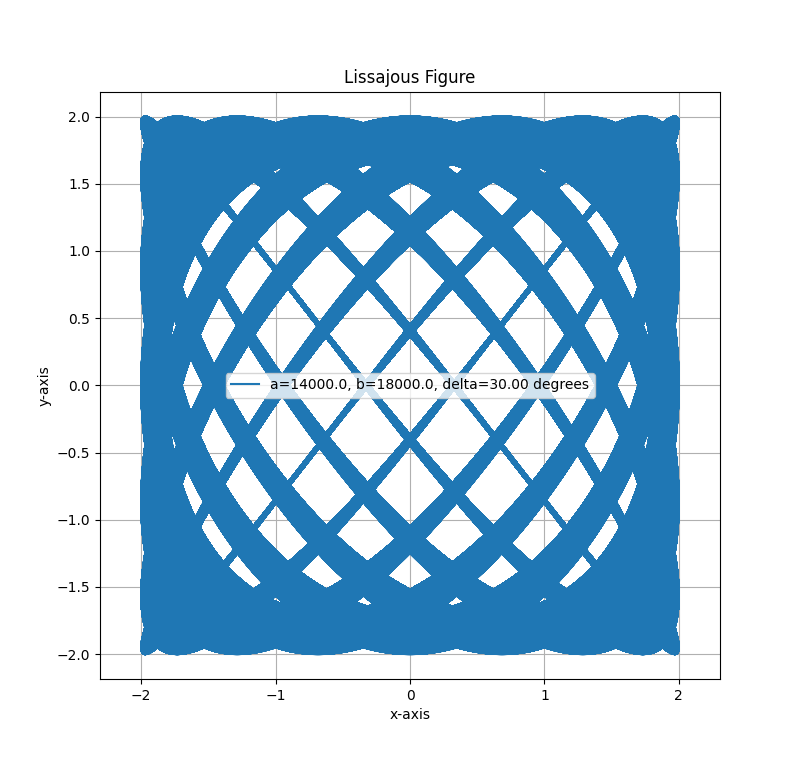
\includegraphics[height=5cm]{figures/6/Figure_6.png}
    \end{subfigure}%
\end{figure}
\section*{\color{myblue}Python Code for verifying the lissajous figures}
Below code can be used to verify the lissajou's figure
\begin{lstlisting}
import numpy as np
import matplotlib.pyplot as plt

def lissajous_figure(A, B, a, b, delta, t_max=2*np.pi, num_points=100000):
    """
    Generate and plot a Lissajous figure.

    Parameters:
        A (float): Amplitude of the sine wave along the x-axis.
        B (float): Amplitude of the sine wave along the y-axis.
        a (float): Ratio of frequencies along the x-axis.
        b (float): Ratio of frequencies along the y-axis.
        delta (float): Phase difference between the two waves (in radians).
        t_max (float): The maximum value of t to plot (default is 2*pi).
        num_points (int): Number of points to plot (default is 1000).
    """
    # Generate time points
    t = np.linspace(0, t_max, num_points)

    # Compute x and y
    x = A * np.sin(a * t + delta)
    y = B * np.sin(b * t)

    # Plot the figure
    plt.figure(figsize=(8, 8))
    plt.plot(x, y, label=f"a={a}, b={b}, delta={np.degrees(delta):.2f} degrees")
    plt.title("Lissajous Figure")
    plt.xlabel("x-axis")
    plt.ylabel("y-axis")
    plt.axis("equal")
    plt.legend()
    plt.grid(True)
    plt.show()

# Example usage
if __name__ == "__main__":
    # Ask user for parameters
    print("Phase difference (delta) should be entered in degrees.")
    A = float(input("Enter amplitude along x-axis (A): "))
    B = float(input("Enter amplitude along y-axis (B): "))
    a = float(input("Enter frequency ratio along x-axis (a): "))
    b = float(input("Enter frequency ratio along y-axis (b): "))
    delta_degrees = float(input("Enter phase difference in degrees (delta): "))
    delta = np.radians(delta_degrees)  # Convert degrees to radians

    lissajous_figure(A, B, a, b, delta)
\end{lstlisting}

\subsection*{\color{myred}Capturing a One-Time Event}
\begin{enumerate}
    \item Set the CRO to "Single Trigger" mode.
    \item Adjust the trigger level and slope (positive or negative).
    \item Connect the one-time signal source to the CRO's input.
    \item Once the event occurs, the CRO freezes the display for analysis.
\end{enumerate}
\begin{figure}[H]
    \centering
    \begin{subfigure}{\textwidth}
        \centering
        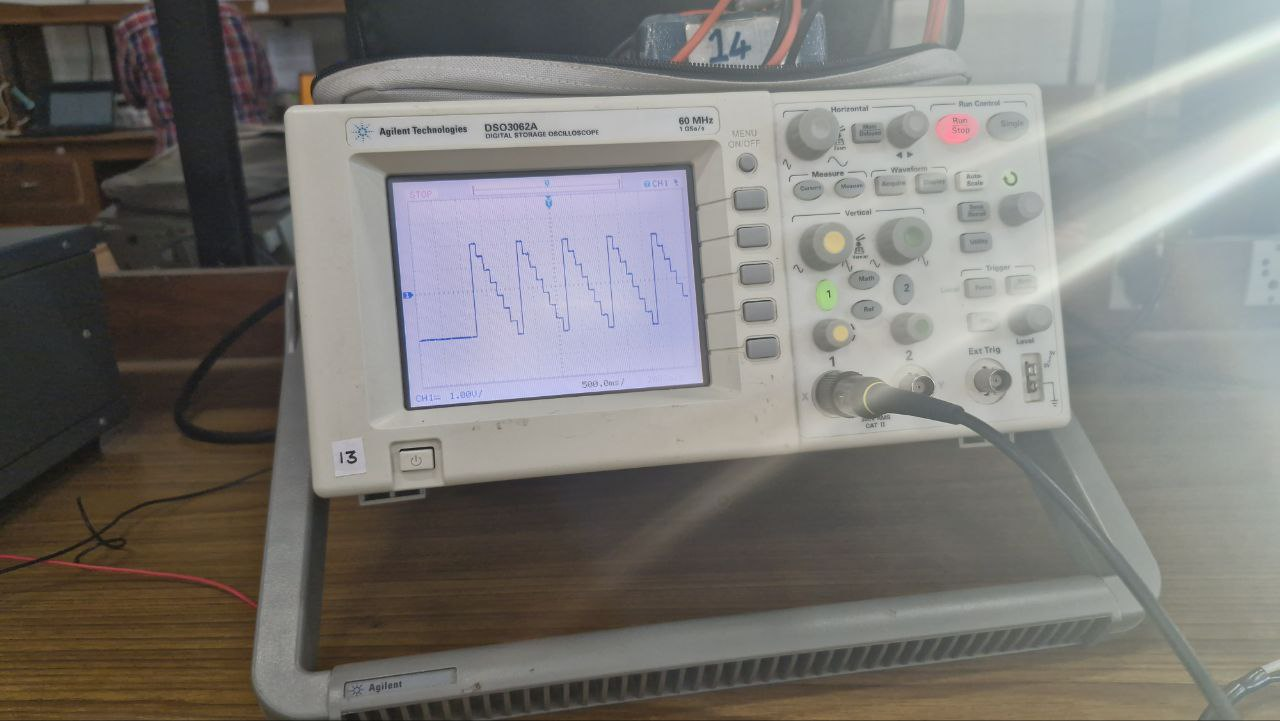
\includegraphics[height=5cm]{figures/Capture_the_event/1/plot.jpg}
    \end{subfigure}%
    \begin{subfigure}{\textwidth}
        \centering
        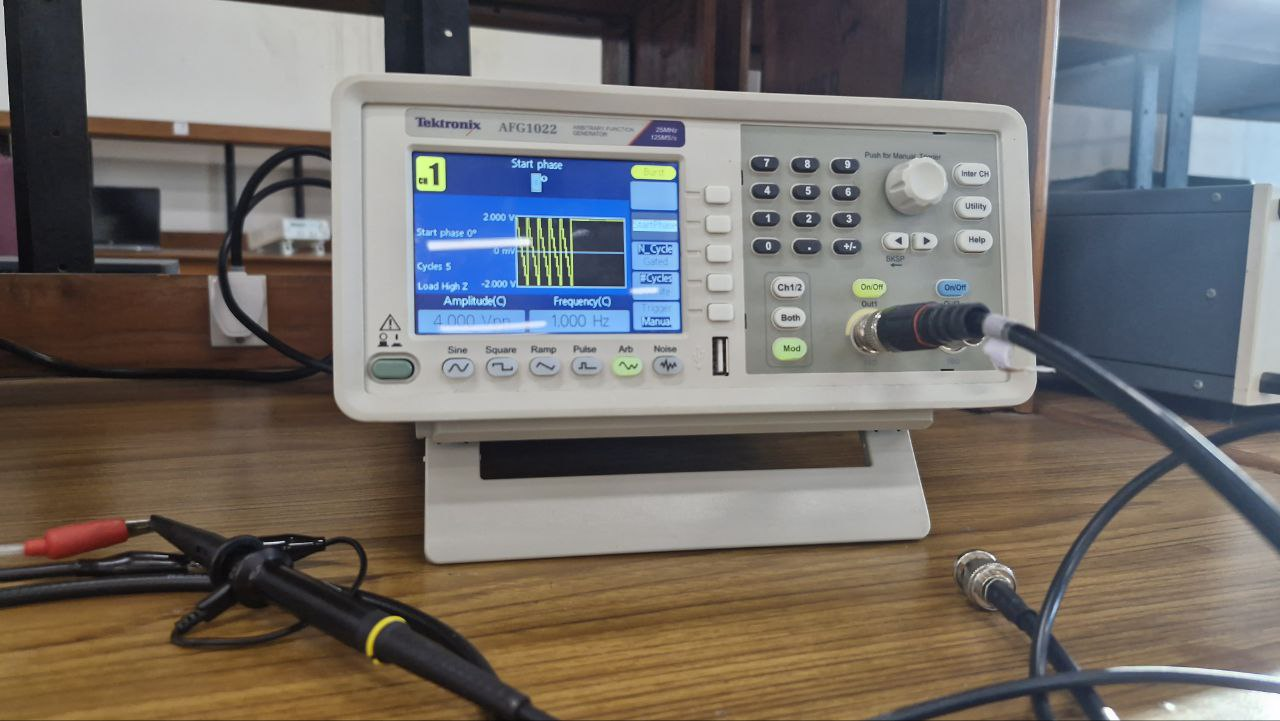
\includegraphics[height=5cm]{figures/Capture_the_event/1/para.jpg}
    \end{subfigure}
\end{figure}
\begin{figure}[H]
    \centering
    \begin{subfigure}{\textwidth}
        \centering
        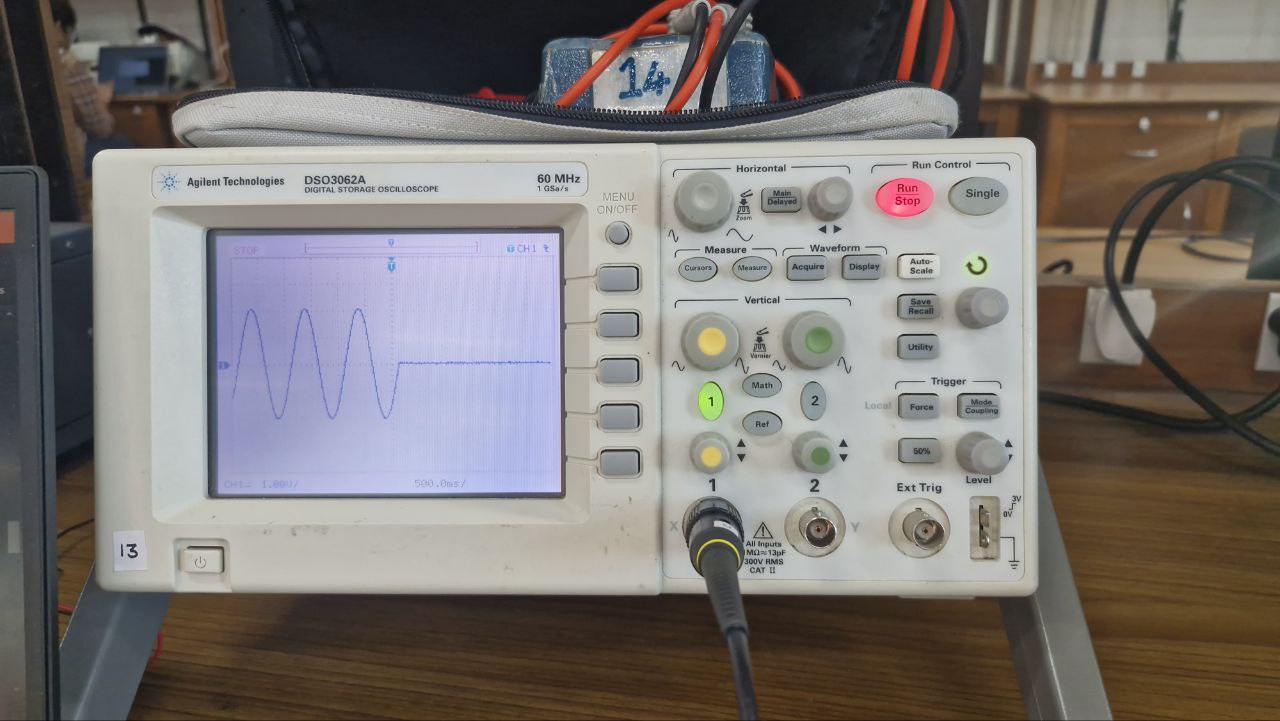
\includegraphics[height=5cm]{figures/Capture_the_event/2/plot.jpg}
    \end{subfigure}%
    \begin{subfigure}{\textwidth}
        \centering
        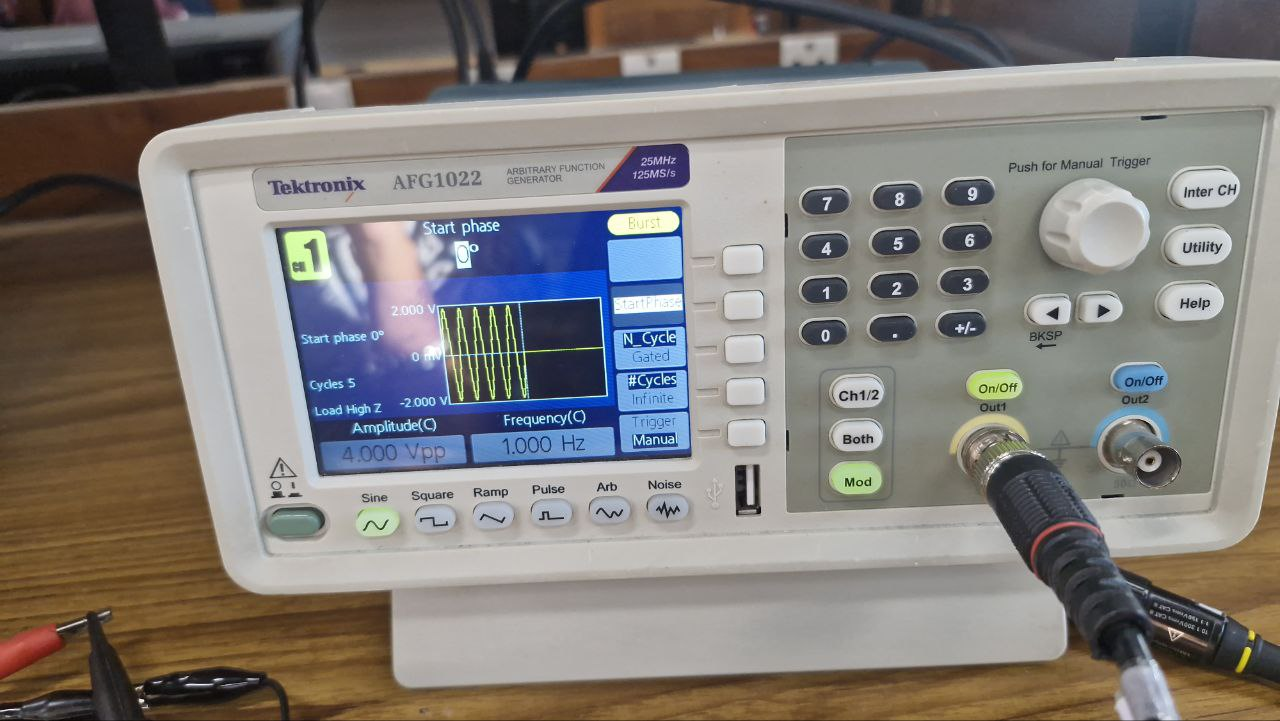
\includegraphics[height=5cm]{figures/Capture_the_event/2/para.jpg}
    \end{subfigure}
\end{figure}
\begin{figure}[H]
    \centering
    \begin{subfigure}{\textwidth}
        \centering
        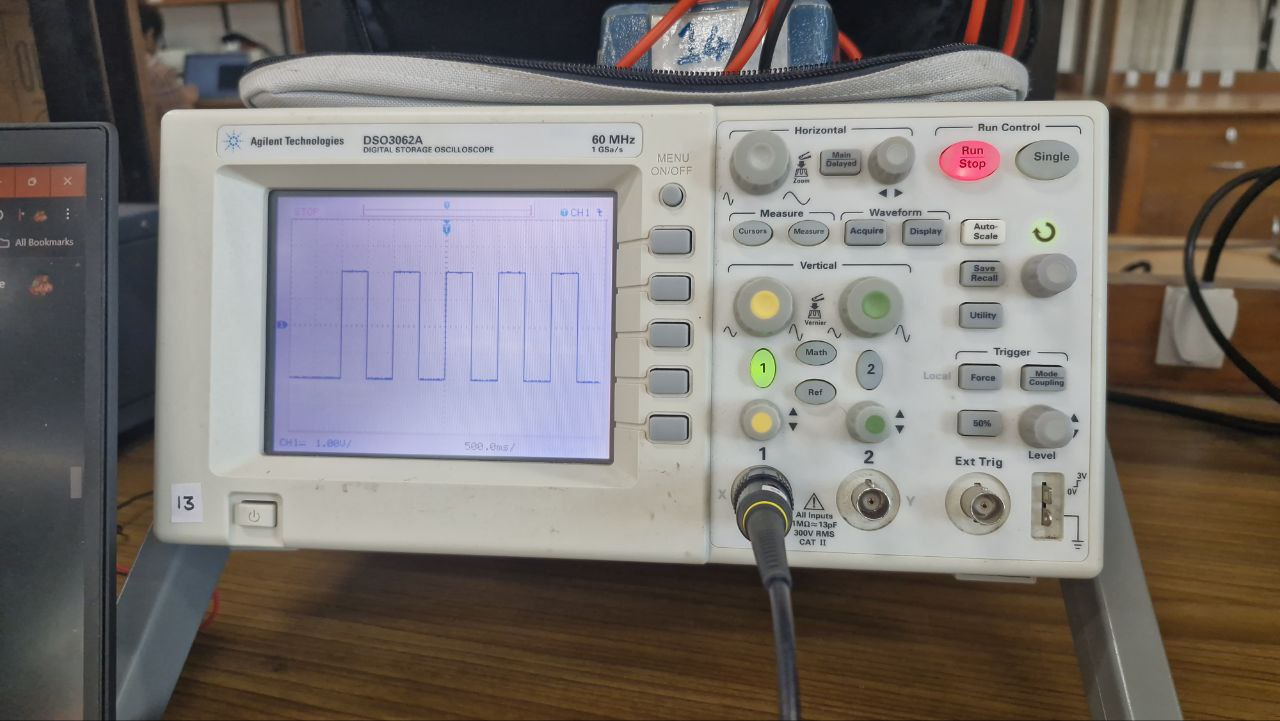
\includegraphics[height=5cm]{figures/Capture_the_event/3/plot.jpg}
    \end{subfigure}%
    \begin{subfigure}{\textwidth}
        \centering
        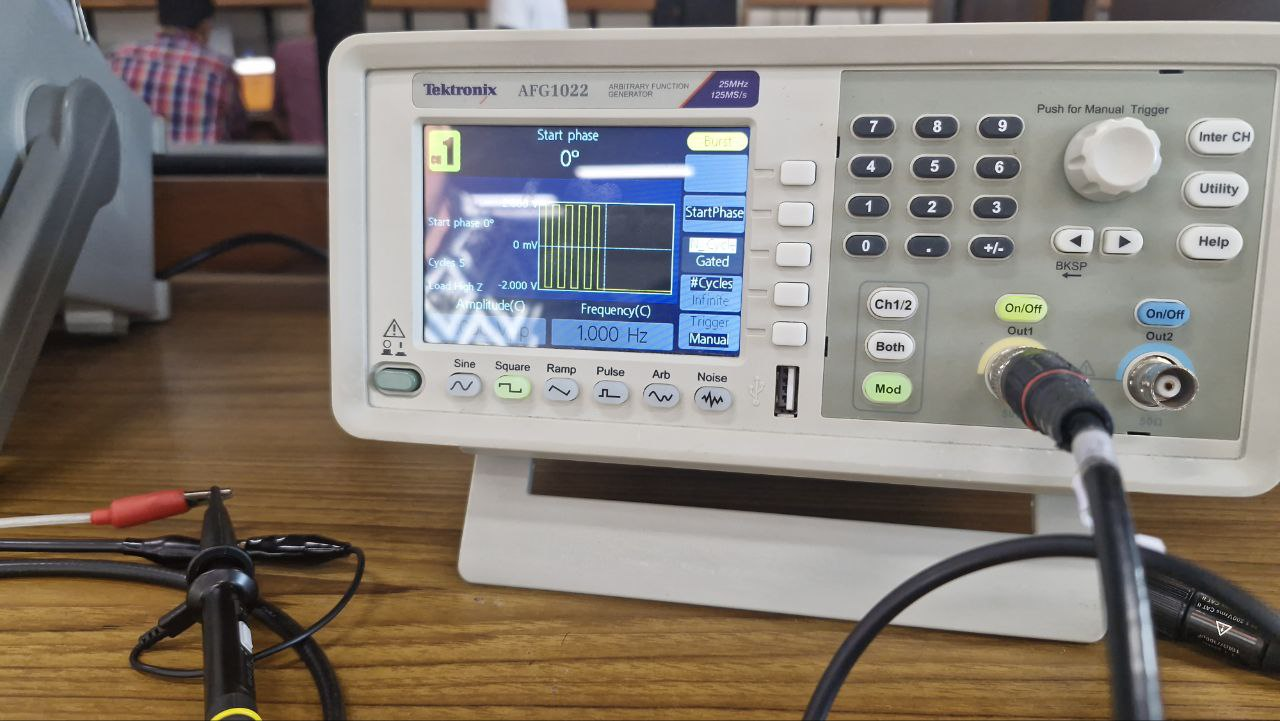
\includegraphics[height=5cm]{figures/Capture_the_event/3/para.jpg}
    \end{subfigure}
\end{figure}

\section*{\color{myblue}Discussion}

\subsection*{\color{mygreen}Lissajous Figures}
\begin{itemize}
    \item The figures provide a visual representation of frequency and phase relationships.
    \item They are especially useful for comparing unknown signal frequencies by matching them against a known reference signal.
\end{itemize}

\subsection*{\color{mygreen}Phase Interpretation}
\begin{itemize}
    \item Variations in the phase difference ($\Delta\phi$) directly affect the symmetry and orientation of the figures.
\end{itemize}

\subsection*{\color{mygreen}Capturing One-Time Events}
CROs with a single-trigger mode are vital for observing transient phenomena like surges or spikes.

\section*{\color{myblue}Conclusion}
\begin{enumerate}
    \item The oscilloscope and function generator together allow precise visualization and analysis of signal waveforms.
    \item Lissajous figures are highly effective for frequency and phase comparison.
    \item CROs can be configured to capture and analyze one-time events using triggering mechanisms.
\end{enumerate}

\end{document}

